\documentclass[11pt]{article} % use larger type; default would be 10pt

\usepackage{tikz}
\usetikzlibrary{calc}
\usetikzlibrary{arrows.meta}

        \newcommand\degree[0]{^{\circ}}

\title{Play with TikZ}
\author{Just Us}
%\date{} % Activate to display a given date or no date (if empty),
         % otherwise the current date is printed 

\begin{document}
\maketitle

\section{Chap 2}
grid

grid-8-8
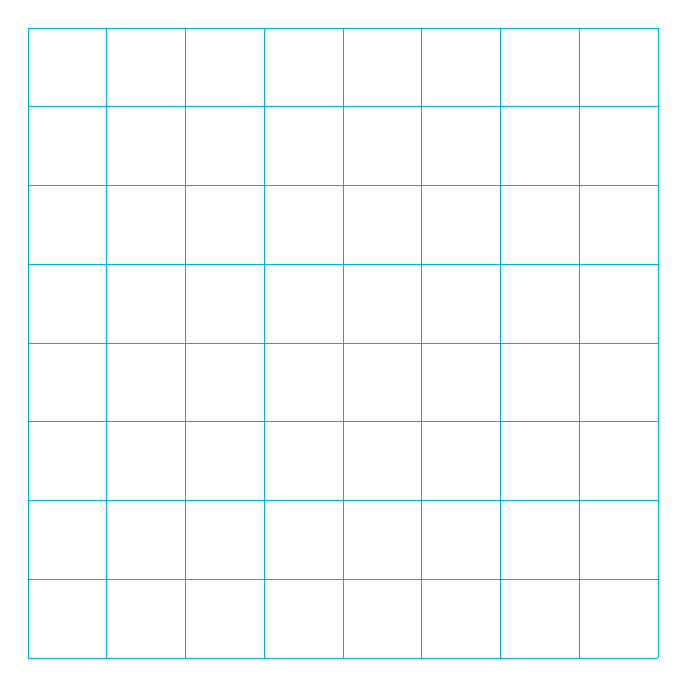
\begin{tikzpicture}

\draw[step=1cm,cyan,very thin] (0,0) grid (8,8);

\end{tikzpicture}
\newline

vertical line

\begin{tikzpicture}

\draw[cyan,thick] (0,0) -- (0,3);

\end{tikzpicture}
\newline

horizontal bar

\begin{tikzpicture}

\filldraw[cyan] (0,0) rectangle +(4,.3);

\end{tikzpicture}
\newline


Exercise not used?
\begin{tikzpicture}
\coordinate (O) at (0,0);
\coordinate (A) at (0,0);
\coordinate (B) at (0,0);
\coordinate(C) at (0,0);
\coordinate (D) at (0,0);
\filldraw[black] (O) circle (.2pt) node[anchor=south west, xshift=6]{$50\degree$};
\filldraw[black] (A) circle (.2pt) node[anchor=south east]{$x$};
\filldraw[black] (B) circle (.2pt) node[anchor=north east, xshift=-6]{$y$};
\filldraw[black] (C) circle (.2pt) node[anchor=north west]{$z$};
%\draw[black,  thick] (A) -- (B) --( C) -- cycle;
\draw[black] (-2.3,0) --  (2.3,0);
\draw[black] (0.8,1.3) --  (-0.8,-1.3) ;
\end{tikzpicture}
\newline


\end{document}
